\documentclass[utf8]{beamer}
\graphicspath{{../../common/icons/}{pics/}{plots/}}

\usepackage{beamerthemesplit}
%\usepackage[ngerman]{babel}
\usepackage{babel}
\usepackage{url}

\usepackage{eurosym}


\usepackage{cite}
\usepackage{color}
\usepackage[justification=centering,figurename=Abb.]{caption}

%\usepackage{bibgerm}
\usepackage{wrapfig}

\usepackage{mathenv, 
			amssymb, 
			amsfonts,
			upgreek, 
			empheq,amsxtra,mathbbol,mathrsfs,dsfont}


\usepackage{graphicx}
\usepackage{enumerate}
\usepackage{array}
\usepackage{pdfpages}

\usepackage{multimedia} %\movie[height=3.5cm, width=4.8cm]{movie-label}{moviefile.avi}
\usepackage{hyperref}

\usepackage{forloop}

\setbeameroption{show notes}
% \usetheme{Boadilla}
%\useinnertheme[shadow=true]{}
%\useoutertheme{smoothbars}

\usepackage{beamerthemesplit}
\usetheme{Frankfurt}             % es gibt noch andere Themen
\usecolortheme{seahorse}

% \usebackgroundtemplate{\includegraphics[width=\paperwidth,height=\paperheight]{test}}
% \setbeamertemplate{footline}[frame number]

%navi aus
\beamertemplatenavigationsymbolsempty
\setbeamercovered{transparent}

\setbeamertemplate{itemize pro}{
\includegraphics[width=3mm]{pro}}
\setbeamertemplate{itemize contra}{
\includegraphics[width=3mm]{contra}}

% Pro / Contra-Items
\newcommand{\pro}{\item[\usebeamertemplate{itemize pro}]}
\newcommand{\contra}{\item[\usebeamertemplate{itemize contra}]}

\newenvironment{ergo}{\vspace{3mm}\begin{minipage}{8mm}
\includegraphics[width=7mm]{arrow-right}\end{minipage}\hspace{2mm}\begin{minipage}{9.5cm}}{\end{minipage}}

\setbeamercolor{note}{fg=black,bg=yellow} 


% \AtBeginSection[]{%
% \begin{frame}
% \tableofcontents[currentsection]
% \end{frame}
% }% AtBeginSection


% Umdefinition der Fußzeile
 \setbeamertemplate{footline}
 {%
 	\leavevmode%
 	\hbox{\begin{beamercolorbox}[wd=.9\paperwidth,ht=2.5ex,dp=1.125ex]{author in head/foot}%
 	\usebeamerfont{author in head/foot}\centering\insertshorttitle
 	\end{beamercolorbox}%
 	\begin{beamercolorbox}[wd=.1\paperwidth,ht=2.5ex,dp=1.125ex,leftskip=.3cm ,rightskip=.3cm plus1fil]{title in head/foot}%
 	\usebeamerfont{title in head/foot}\hfill\insertframenumber/\inserttotalframenumber
 	\end{beamercolorbox}}%
 	\vskip0pt%
 }
 
\newcommand{\entspricht}{\mathrel{\widehat{=}}}


\renewcommand{\theequation}	{\thesubsection.\arabic{equation}} 
\renewcommand{\thefigure}	{\thesubsection.\arabic{figure}}
\renewcommand{\thetable}	{\thesubsection.\arabic{table}}

\makeatletter
	\@addtoreset{equation}{section}
  	\@addtoreset{figure}{section}
  	\@addtoreset{table}{section}

  	\renewcommand{\@fnsymbol}[1]{\ensuremath{%
  	\ifcase#1\or *\or **\or {**}*\or
	\mathsection\or \mathparagraph\or \|\or \star\or
	\star\star\or {\star\star}\star \else\@ctrerr\fi}}
   	%\ renewcommand macht bei Thanks das Dagger zu **
\makeatother


\newenvironment{changemargin}[2]{%
\begin{list}{}{%
\setlength{\topsep}{0pt}%
\setlength{\leftmargin}{#1}%
\setlength{\rightmargin}{#2}%
\setlength{\listparindent}{\parindent}%
\setlength{\itemindent}{\parindent}%
\setlength{\parsep}{\parskip}%
}%
\item[]}{\end{list}}



\newcommand{\beginbackup}{
   \newcounter{framenumbervorappendix}
   \setcounter{framenumbervorappendix}{\value{framenumber}}
}
\newcommand{\backupend}{
   \addtocounter{framenumbervorappendix}{-\value{framenumber}}
   \addtocounter{framenumber}{\value{framenumbervorappendix}} 
}




\usepackage[ngerman]{babel}
\usepackage{bibgerm}

	
%\title{Design and Development of the Software and Computing Framework for the
%L1/L2 Online PC Farm of the NA62 Experiment at CERN}
\title{Design of the Online PC Farm for the High Level Trigger of the NA62 Experiment at CERN}

\author{Jonas Kunze}
\date{11/1/2012\newline\tiny IEEE NSS Anaheim, California}

\institute[{Universität Mainz}]{
	\inst{} University of Mainz}
\titlegraphic{
\includegraphics[height=3cm]{penguins}}
\logo{
\includegraphics[width=2cm]{na62-logo}}
\subject{NA62 online pc-farm design and implementation}
\keywords{NA62,computing,multithreading,trigger,c++,boost,asio,10g}

 \AtBeginSection[]{%
 \begin{frame}
 \tableofcontents[currentsection]
 \end{frame}
 }% AtBeginSection

\begin{document}
  	\frame{
  		\titlepage
  		\vspace{-2cm}
  		
\includegraphics[width=0.2\textwidth]{bmbf-logo}
  		\vspace{1cm}
  	}
  	
  	\frame{\tableofcontents}
  	\section{Motivation}
\subsection{The physics}
\begin{frame}{}{}
	\begin{columns}
	 	\column{.3\textwidth}
	 		\begin{center} 
				
\includegraphics[height=4cm]{penguino}
			\end{center}
	    \column{.65	\textwidth}
	    	\begin{block}{$K^+ \rightarrow \pi^+ \nu \bar{\nu} ~\Leftrightarrow ~
	    	V_{td}$ of CKM matrix} SM branching ratio: $(8.5\pm 0.7)\cdot 10^{-11}$
			\end{block}
			\begin{block}{Measurement from BNL (Brookhaven)}
				The only experimental data so far (7 candidates)
	    		E787 and E949:\\
	    		$BR(K^+ \rightarrow \pi^+ \nu \bar{\nu})=(17.3^{+11.5}_{-10.5})\cdot
	    		10^{-11}$
			\end{block}
			\begin{exampleblock}{NA62 aims $\sigma < 10\%$ with 100 events}
	    		$\approx 10^{13} ~ K^+$ decays required
			\end{exampleblock}
	\end{columns}
	\begin{block}{High efficiency needed $\Rightarrow$ high data rate}
		Signal-to-noise ratio of 1/10 planned with an event rate of 10 MHz
	\end{block}
\end{frame}

\begin{frame}{Background channels to be suppressed by the detector}{}
	\begin{align*}
	   K^+ &\rightarrow \mu^+ \nu &(63\%) &\rightarrow \mu \text{ veto} \\
		 K^+ &\rightarrow \pi^+ \pi^0 &(21\%) &\rightarrow \gamma \text{ veto} \\
	  	 K^+ &\rightarrow \pi^+ \pi^+ \pi^- &(6\%) &\rightarrow \text{charged particle veto} \\
	  	 K^+ &\rightarrow \pi^0 e^+ \nu &(5\%) &\rightarrow \gamma \text{ veto}  \\
	  	  K^+ &\rightarrow \pi^0 \mu^+ \nu &(3\%) &\rightarrow \gamma, \mu \text{ veto} \\
	  	   K^+ &\rightarrow \pi^+ \pi^0 \pi^0 &(2\%) &\rightarrow \gamma \text{
	  	  veto}		  	
	\end{align*}
	\begin{ergo}
		Detector dominated by vetos
	\end{ergo}
\end{frame}

\section{The experiment}
\subsection{Subdetectors}
\begin{frame}{Experiment overview}{}
	\begin{center} 
		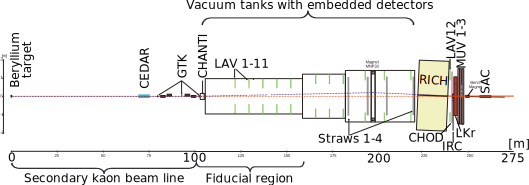
\includegraphics[width=\textwidth]{na62-overview}
	\end{center}
\end{frame}

\begin{frame}{CEDAR}{}
	\begin{center} 
		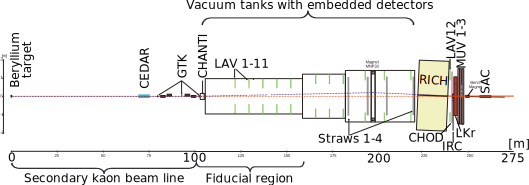
\includegraphics[width=\textwidth]{na62-overview}
	\end{center}
	\begin{block}{Differential Cerenkov counter}
		$K^+$ identification \\
		Mirrors collect $K^+$-specific Cerenkov light
	\end{block}
\end{frame}

\begin{frame}{GTK}{}
	\begin{center} 
		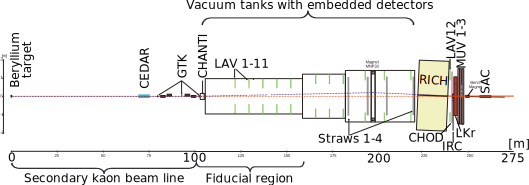
\includegraphics[width=\textwidth]{na62-overview}
	\end{center}
	\begin{block}{Gigatracker (second Achromat)}
		Timing, momentum and angle of all particles using silicon pixels \\
		750 MHz event rate!!!
	\end{block}
\end{frame}

\begin{frame}{Straws}{}
	\begin{center} 
		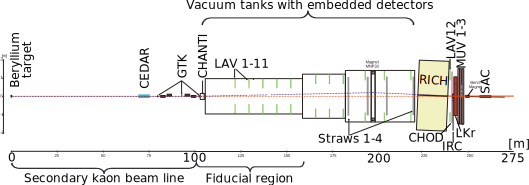
\includegraphics[width=\textwidth]{na62-overview}
	\end{center}
	\begin{block}{Spectrometer}
		Tracking of charged particles within a magnetic field
	\end{block}
\end{frame}

\begin{frame}{Photon vetos part 1: LAV, IRC, SAC}{}
	\begin{center} 
		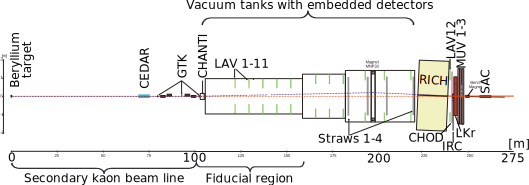
\includegraphics[width=\textwidth]{na62-overview}
	\end{center}
	\begin{block}{Photon vetos}
		Huge range of angle to be covered \\ 
		Scintillators at different positions (lead-glass reused from OPAL)
	\end{block}
\end{frame}

\begin{frame}{Photon veto part 2: LKr}{}
	\begin{center} 
		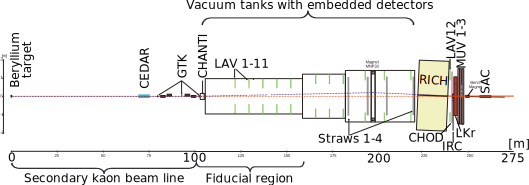
\includegraphics[width=\textwidth]{na62-overview}
	\end{center}
	\begin{block}{Liquid Krypton calorimeter}
		Photon veto for central angles range\\
		Muon veto \\
		Reused from NA48 $\Rightarrow$ can be used as calorimeter for analysis of
		additional rare decays
	\end{block}
\end{frame}

\begin{frame}{Rich}{}
	\begin{center} 
		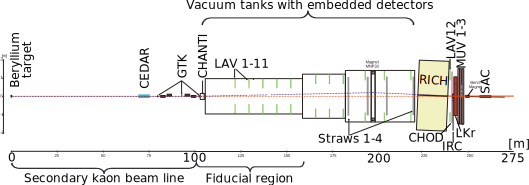
\includegraphics[width=\textwidth]{na62-overview}
	\end{center}
	\begin{block}{Ring Imaging Cherenkov}
		Separate $\pi^+$ from $\mu^+$ between 15 and 35 GeV/c (L0 trigger)
	\end{block}
\end{frame}



\begin{frame}{MUV}{}
	\begin{center} 
		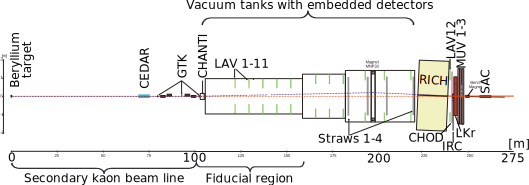
\includegraphics[width=\textwidth]{na62-overview}
	\end{center}
	\begin{block}{Muon veto}
		Scintillator-iron-sandwich mainly produced in Mainz 
	\end{block}
\end{frame}

% \begin{frame}{Subdetector functionalities}{}
% \begin{description}
%   \item[CEDAR] Differential Cerenkov counter for Kaon tagging
%   \item[GTK] Timing, momentum, angle of all hadrons
%   \item[CHANTI] Detect inelastic interactions in GTK ($K^+ \rightarrow \pi^+
%   \pi^0$)
%     \item[LAV] Large angle photon veto
%     \item[LKr] Medium angle photon veto
%     \item[IRC \& SAC] Small angle photon veto  
%    	\item[STRAW] Direction and momentum of charged particles
%    	\item[RICH] Ring Imaging Cherenkov for vetoing muons
%    	\item[CHOD] Charged hodoscope for low energy hadrons from photonuclear
%    	interactions
%    	\item[MUV] Muon Veto
% \end{description}
% \end{frame}

\begin{frame}{Data rates}{}
	\begin{center}
		\textbf{10 MHz unsteady $K^+$ rate}
	\end{center}
	\begin{table}[H]
		\begin{center}
			\begin{tabular}{c|c|>{\centering\arraybackslash}m{3cm}}
			Detector	&	Event size [B] &	Data rate [GBps]\\
			\hline
			CEDAR	&	216		&	2.16	\\
			GTK 	&	2250	&	22.50 	\\
			CHANTI	&	192		&	1.92 	\\
			LAV 	&	160		&	1.60 	\\
			STRAW 	&	768		&	7.68 	\\
			RICH 	&	160		&	1.60 	\\
			CHOD	&	$\ll1000$	&	$\ll10$\\
			MUV 	&	768		&	7.68 \\
			IRC \& SAC 	& 576	& 	5.76 	\\
			\textbf{LKR}		&	\textbf{222~k}	&	\textbf{2220}	\\
			\hline
			\textbf{Sum}	&	\textbf{$\approx$227~kB}	&	\textbf{$\approx$2.3~TBps}\\
			\end{tabular}
		\end{center}
	\end{table}
\end{frame}
  	\section{Trigger topology}

\subsection{Three level online trigger}
\begin{frame}{Online trigger system}{Three levels to filter data}
	Data transmission via ordinary 10 gigabit ethernet and \textbf{UDP/IP}:
	\begin{center} 
		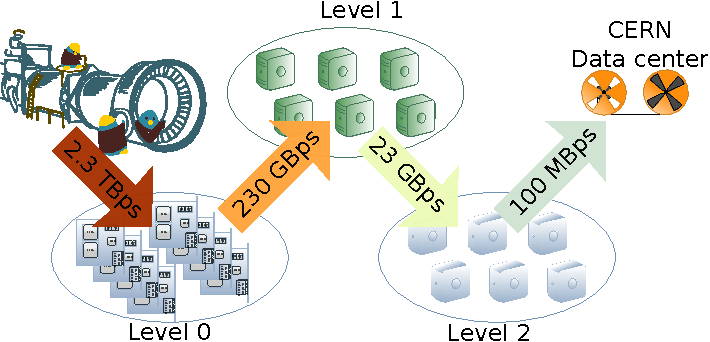
\includegraphics[width=\textwidth]{data-mitigation}
	\end{center}
\end{frame}

\begin{frame}{First topology proposal}{}
	Original concept:
	\begin{center} 
		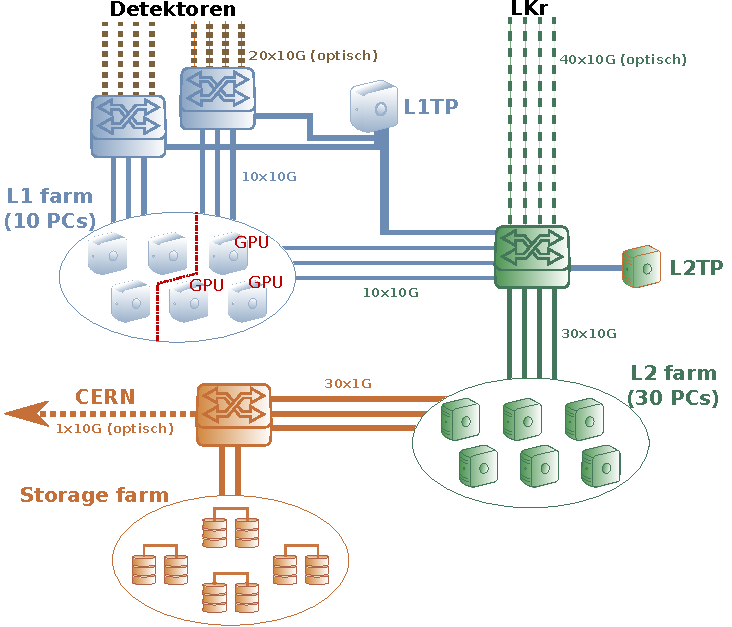
\includegraphics[width=0.7\textwidth]{double-star}
	\end{center}
\end{frame}

\subsection{New proposal}
\begin{frame}{Burst time}{}
	\vspace{-2mm}
	\begin{block}{}
		Only 3-9 sec. proton burst and long break
	\end{block}

	\begin{figure}[htp]
		\begin{center}
		  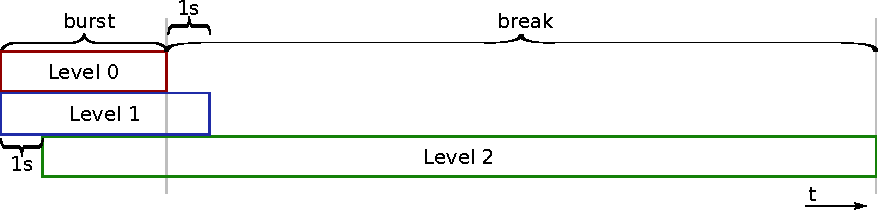
\includegraphics[width=\textwidth]{bursttime-engl}
		  %\caption{Original approach}
		\end{center}
	\end{figure}
	
	\vspace{-5mm}
	\begin{exampleblock}{My proposal to use resources more efficiently}<2->
		Combine L1 and L2 to one farm
	\end{exampleblock}

	\begin{figure}[htp]
		\begin{center}
		 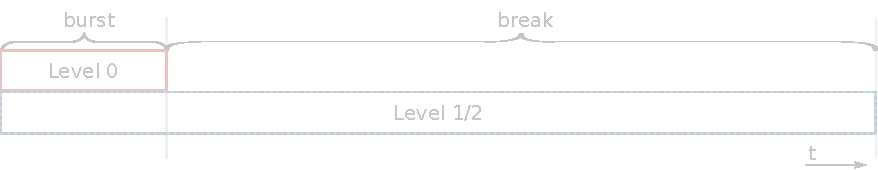
\includegraphics[width=\textwidth]{bursttime-l12merged-engl-light}<1>
		 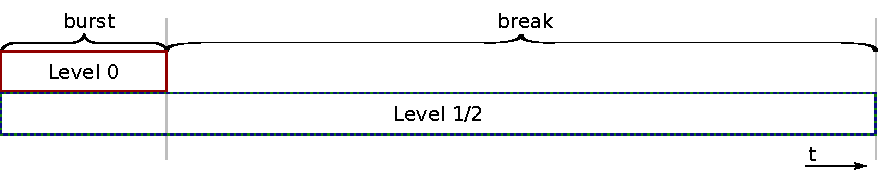
\includegraphics[width=\textwidth]{bursttime-l12merged-engl}<2->
		\end{center}
	\end{figure}
\end{frame}

\begin{frame}{Don't separate L1 and L2!}{}
	\begin{center} 
		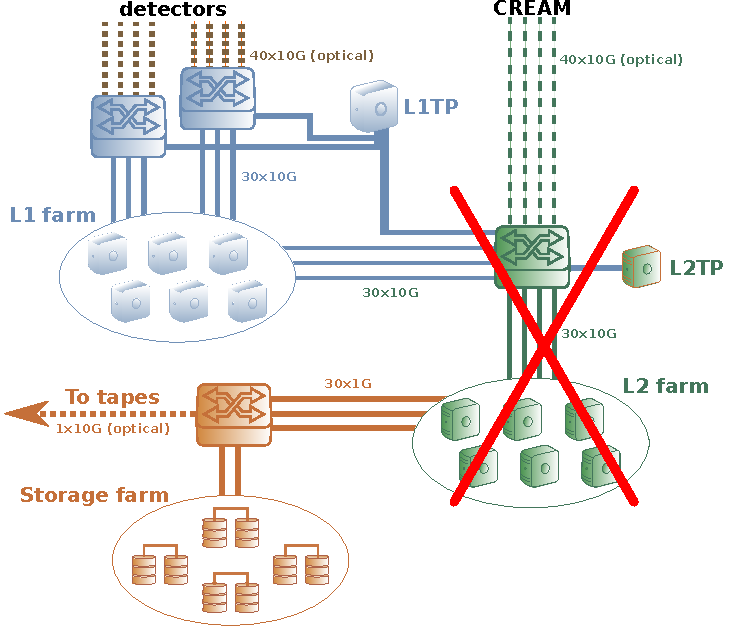
\includegraphics[width=0.8\textwidth]{whole-farm-nol2}
	\end{center} 
\end{frame}

\begin{frame}{Combine L1 and L2 to one farm}{}
	\begin{center} 
		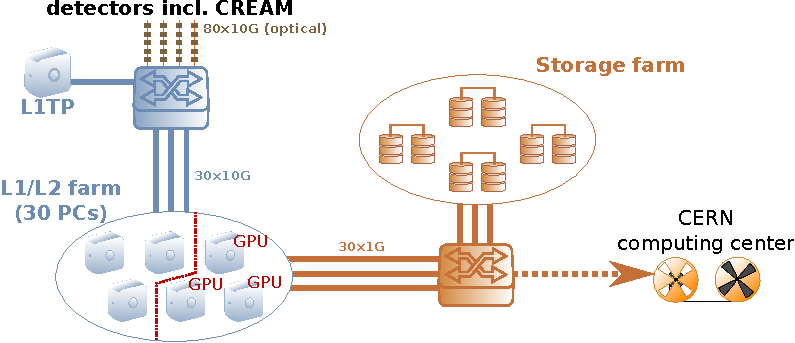
\includegraphics[width=0.9\textwidth]{merged-star}
	\end{center} 
	\begin{exampleblock}{We save about 80k€}
		\begin{itemize}
		  \item No L1 PCs anymore
		  \item Less switches, less network cards
		\end{itemize}
	\end{exampleblock}
\end{frame}

\begin{frame}{New proposal}{Event building @ L1}
	\begin{center} 
		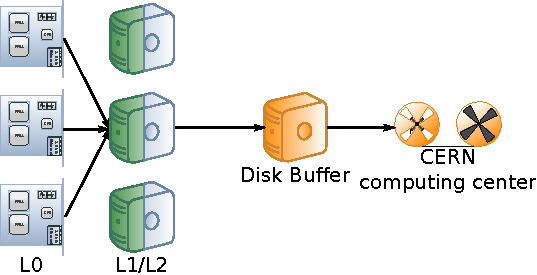
\includegraphics[width=0.6\textwidth]{dataflow-merged-gian-engl}
	\end{center} 
	
	\begin{block}{Every subdetector sends data of one event to the same PC}
		\begin{itemize}
		  	\pro \textbf{More physics at earlier state}
		  	\pro No broadcast of a L1 decision needed anymore
		  	\pro Easier to implement load balancing (self-sustaining PCs)
%  			\contra Every farm PC must serve every subdetector $\Rightarrow$ needs
  			% GPUs
		\end{itemize}
	\end{block}
\end{frame}

  	\section{Performance}

\begin{frame}{pf\_ring - new type of network socket}{}
	\begin{alertblock}{Bad performance with standard Kernel sockets}
		Interrupt based	transmission causes packet loss
	\end{alertblock}
	
	\begin{block}{Special socket: pf\_ring DNA by ntop}
		\begin{itemize}
		  \item Direct access to the NIC memory (avoids system calls)
		  \item Only $\approx$40\% CPU @ full speed 10G receiving 1kB packets
		  \item No packet loss at all
		\end{itemize}
	\end{block}
	\begin{ergo}
		270kHz Eventbuilding rate with only 5 virtual cores \\
		$\Rightarrow$ 19 cores left for L1 and L2	trigger
	\end{ergo}
\end{frame}



  	\section{Conclusion}
\begin{frame}{Conclusion}{}
	\begin{itemize}
		\mickey NA62@CERN: search for new physics in $K^+ \rightarrow \pi^+ \nu
		\bar{\nu}$
		
		\vspace{2mm}
		\mickey High precision (BR $< 10^{-10}$) $\Rightarrow$ high data rate
		
		\vspace{2mm}
		\mickey A homogeneous PC farm saves money and work
		
		\vspace{2mm}
		\mickey Using ordinary 10G ethernet saves money but lossless communication only
feasible with special software like pf\_ring DNA
		
	\end{itemize}
\end{frame}


	\begin{frame}{}
		\begin{center}
			\textbf{
\includegraphics[width=0.4\textwidth]{theend}}
		\end{center} 
	\end{frame}
\end{document}